\documentclass[aspectratio=169]{beamer}
\usepackage{amsmath}
\usepackage{amssymb}
\usepackage{amsfonts}
\usepackage{graphicx}
\usepackage{luatexja} 
\usepackage{comment}
\usepackage{bm}
\usepackage{setspace}
\usepackage{caption}

\usetheme{LightTheme}
\setbeamertemplate{footline}[frame number]
\setbeamertemplate{navigation symbols}{}
\setlength{\baselineskip}{10pt}
\begin{document}

% タイトルフレーム
\title{進捗状況}
\subtitle{React\ Hook} 
\author{\small B4 小林紹子} % 必要に応じて変更・削除
\date{\small\today} % 必要に応じて変更・削除

\begin{frame}
    \titlepage
\end{frame}

\begin{frame}{目次}
    \tableofcontents
\end{frame}

\section{React\ Hook}

\begin{frame}{useCallback}
    \begin{itemize}
        \setlength{\itemsep}{2em}
        \item useCallbackは関数をメモ化するためのフック.
        \item useCallbackの第一引数は関数で,第二引数は依存配列.
        \item 関数の再描画が行われる際に,useCallback()は依存配列の中の値を比較.
        \item 依存配列の値がそれぞれ同じ場合は,useCallback()はメモ化している関数を返す.
        \item 異なる場合は,現在の第一引数の関数をメモに保存する.\rightarrowfill 新しい関数を返す.
    \end{itemize}
\end{frame}

\begin{frame}{memo関数とuseCallbackの関係}
    \begin{itemize}
        \setlength{\itemsep}{2em}
        \item memo関数
        \begin{itemize}
            \item propsが同じであれば再描画をスキップする.
        \end{itemize}
        \item useCallback
        \begin{itemize}
            \item 関数の参照をメモ化.
            \item 依存配列が変わらない限り,同じ関数オブジェクトを再利用.
            \item 再レンダーされても「新しい関数が作られる」ことはない.
        \end{itemize}
    \end{itemize} 
    \rightarrowfill useCallbackとmemo関数を同時に使うことで再描画を防げる.

\end{frame}
\begin{frame}
    \begin{figure}
        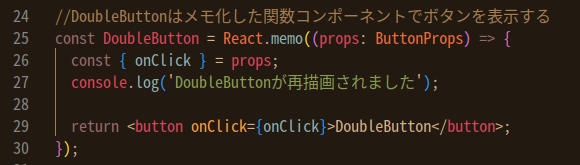
\includegraphics[scale = 0.5]{useCallback1.png}
    \end{figure}
    \begin{figure}
        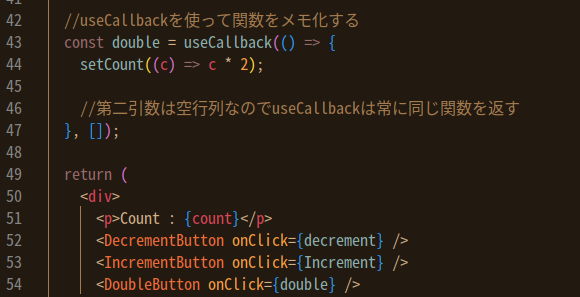
\includegraphics[scale = 0.5]{useCallback2.png}
    \end{figure}
\end{frame}


\end{document}


